\begin{frame}[t,plain]
    \titlepage
\end{frame}

%%%%%%%%%%%%%%%%%%%%%%%%%%%%%%%%%%%%
%%%%%%%%%%%%%%%%%%%%%%%%%%%%%%%%%%%%
\begin{frame}{Outline}
    \tableofcontents
\end{frame}

%%%%%%%%%%%%%%%%%%%%%%%%%%%%%%%%%%%%
%%%%%%%%%%%%%%%%%%%%%%%%%%%%%%%%%%%%
\section{Context and Motivation}

%%%%%%%%%%%%%%%%%%%%%%%%%%%%%%%%%%%%
%%%%%%%%%%%%%%%%%%%%%%%%%%%%%%%%%%%%
{
\usebackgroundtemplate{
\includegraphics[height=\paperheight, width=\paperwidth]{figures/world-map.jpg}}
\begin{frame}[c,fragile]{Context}
    \begin{figure}
        \centering
        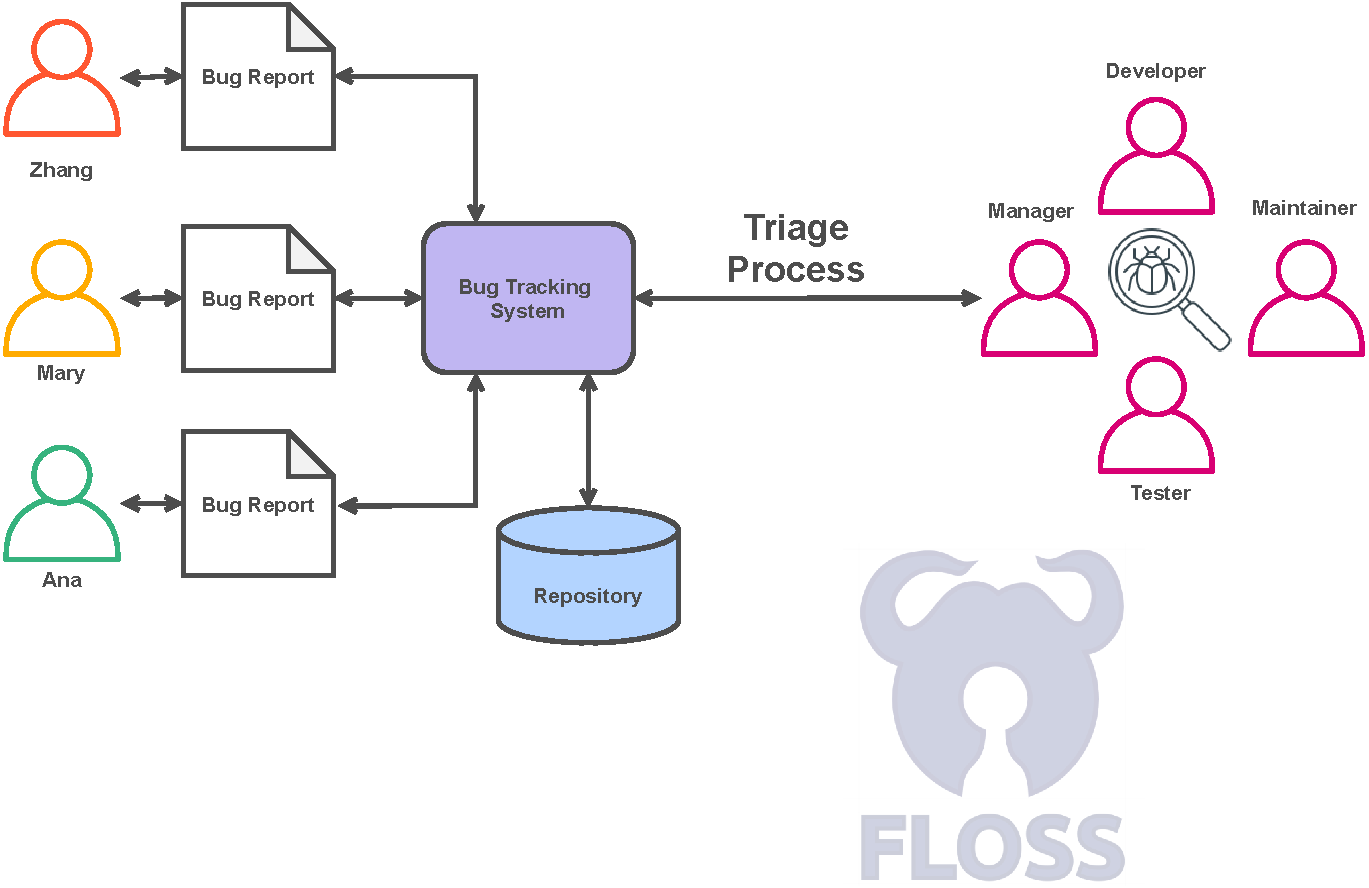
\includegraphics[width=\textwidth]{figures/context-1.pdf}
    \end{figure}
\end{frame}
}

%%%%%%%%%%%%%%%%%%%%%%%%%%%%%%%%%%%%
%%%%%%%%%%%%%%%%%%%%%%%%%%%%%%%%%%%%
\begin{frame}[t,fragile]{Context}
    \vspace{-10pt}
    \begin{figure}
        \centering
        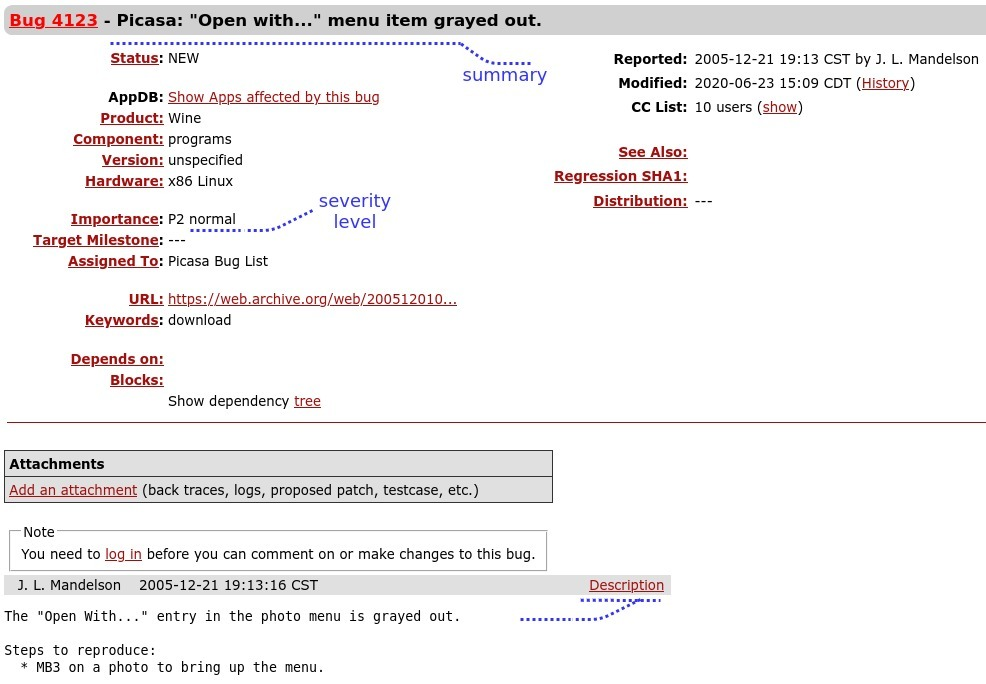
\includegraphics[height=.75\paperheight, width=\textwidth]{figures/exemplo-bug-report-wine-hq.jpg}
    \end{figure}
\end{frame}

{
\pgfdeclareimage[height=\paperheight, width=\paperwidth]{bugreportstress}{figures/bug-report-stress-1.jpg}
\usebackgroundtemplate{\tikz\node[opacity=0.1, inner sep=0]{\pgfuseimage{bugreportstress}};}

%%%%%%%%%%%%%%%%%%%%%%%%%%%%%%%%%%%%

%%%%%%%%%%%%%%%%%%%%%%%%%%%%%%%%%%%%
\begin{frame}[t,fragile]{Triage Process}    
    \begin{columns}[T] % align columns
	    \begin{column}{\textwidth}
			\begin{itemize}
			    \item Bug report duplication
				\item \alert{Severity level assignment}
				\item Assignee allocation
				\item \alert{Bug fix time estimation}
				\item Bug report prioritization
				\end{itemize}
			\end{column}%
		\end{columns}
\end{frame}


%%%%%%%%%%%%%%%%%%%%%%%%%%%%%%%%%%%%
%%%%%%%%%%%%%%%%%%%%%%%%%%%%%%%%%%%%
}

{
\pgfdeclareimage[height=\paperheight, width=\paperwidth]{bugreportstress}{figures/bug-report-stress-2.jpg}
\usebackgroundtemplate{\tikz\node[opacity=0.1, inner sep=0]{\pgfuseimage{bugreportstress}};}
\begin{frame}[t,fragile]{Bug Reports Opened in Eclipse in 2020 } 
	\begin{center}
	    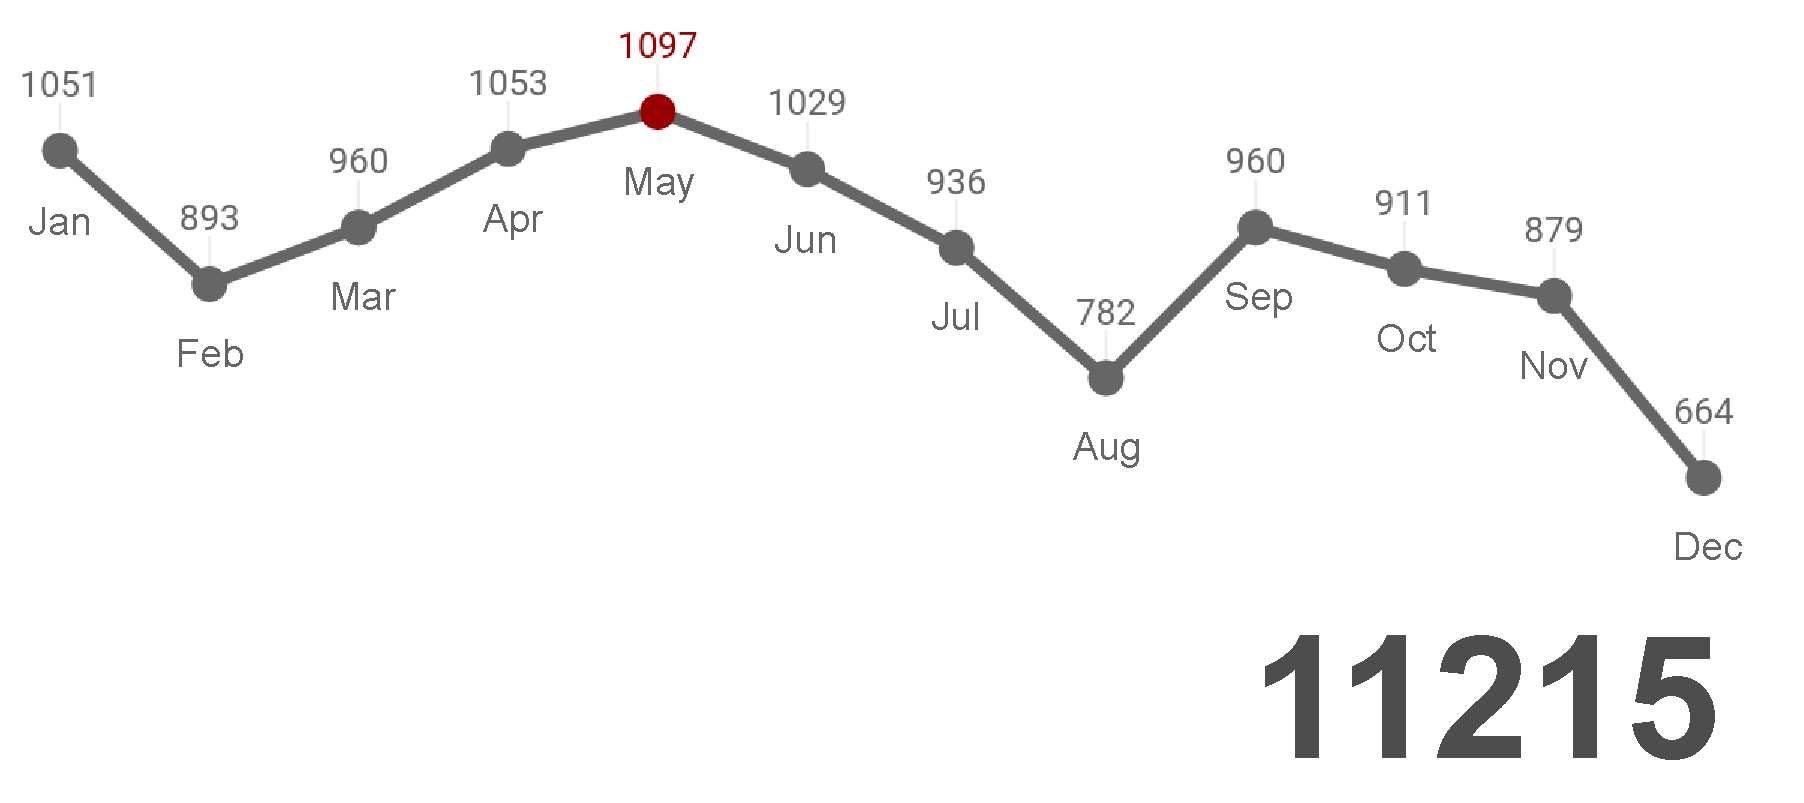
\includegraphics[width=\textwidth]{figures/pdfresizer.com-pdf-crop(1).pdf}
	\end{center}   
\end{frame}
}

%%%%%%%%%%%%%%%%%%%%%%%%%%%%%%%%%%%%
%%%%%%%%%%%%%%%%%%%%%%%%%%%%%%%%%%%%
\begin{frame}[t,fragile]{Motivation}
    \begin{figure}
        \centering
        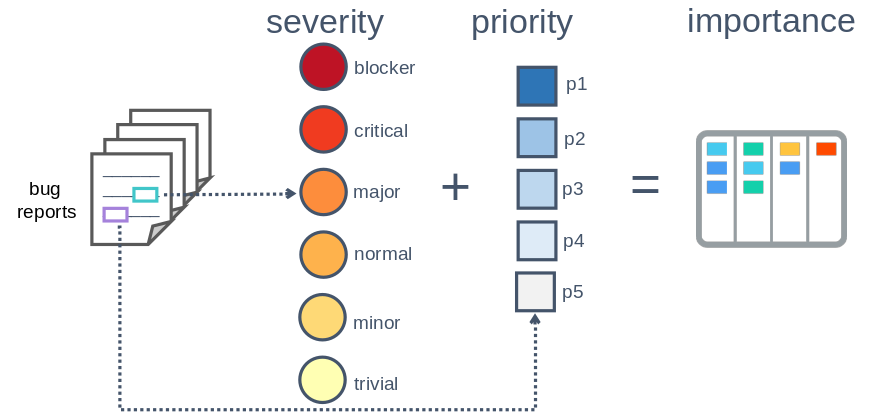
\includegraphics[width=\textwidth]{figures/context-2.png}
    \end{figure}
\end{frame}

%%%%%%%%%%%%%%%%%%%%%%%%%%%%%%%%%%%%
%%%%%%%%%%%%%%%%%%%%%%%%%%%%%%%%%%%%
\begin{frame}[t,fragile]{Motivation}
    \begin{figure}
        \centering
        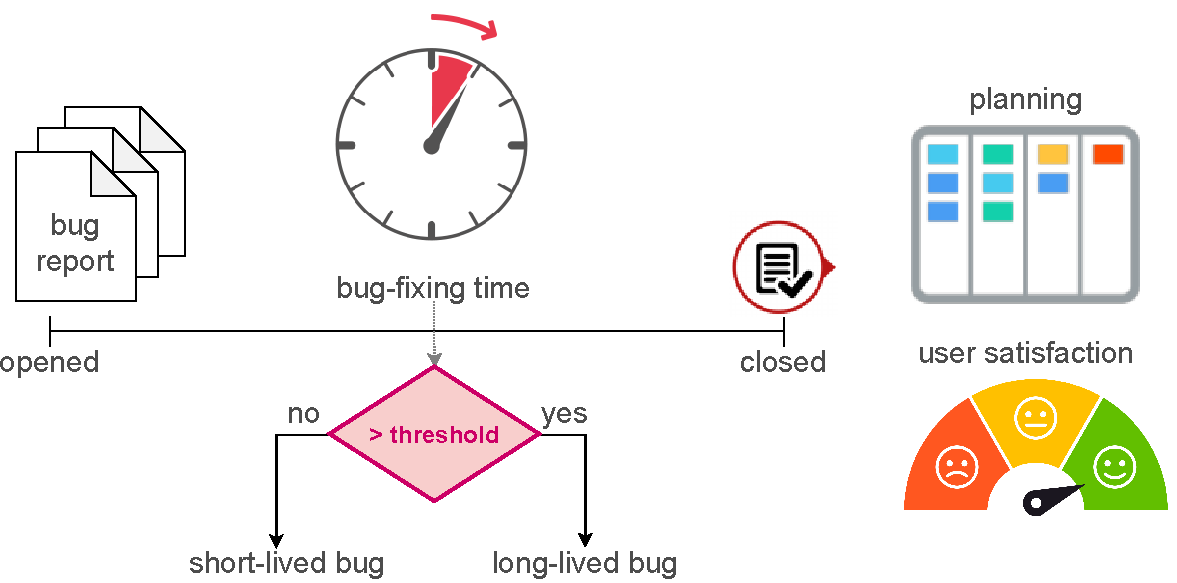
\includegraphics[width=\textwidth]{figures/motivation-2.pdf}
    \end{figure}
\end{frame}

%%%%%%%%%%%%%%%%%%%%%%%%%%%%%%%%%%%%
%%%%%%%%%%%%%%%%%%%%%%%%%%%%%%%%%%%%

\section{Goals 1, 2, and 3}


%%%%%%%%%%%%%%%%%%%%%%%%%%%%%%%%%%%%
%%%%%%%%%%%%%%%%%%%%%%%%%%%%%%%%%%%%
\begin{frame}[t,fragile]{Research Goals}
    \begin{itemize}
        \item \colorbox{RoyalPurple}{\textcolor{White}{Goal 1}}: Understand the \alert{state of the art} in bug \alert{severity level prediction} researching in FLOSS
        \item \colorbox{BurntOrange}{\textcolor{White}{Goal 2}}: Compare traditional ML algorithms in \alert{long-lived bug prediction} in FLOSS
        \item \colorbox{OliveGreen}{\textcolor{White}{Goal 3}}: Evaluate \alert{BERT-based feature extraction} in long-lived bug prediction in FLOSS
    \end{itemize}
\end{frame}

%%%%%%%%%%%%%%%%%%%%%%%%%%%%%%%%%%%%
%%%%%%%%%%%%%%%%%%%%%%%%%%%%%%%%%%%%
\begin{frame}[t,fragile]{Thesis Organization}
	\begin{figure}
		\centering
		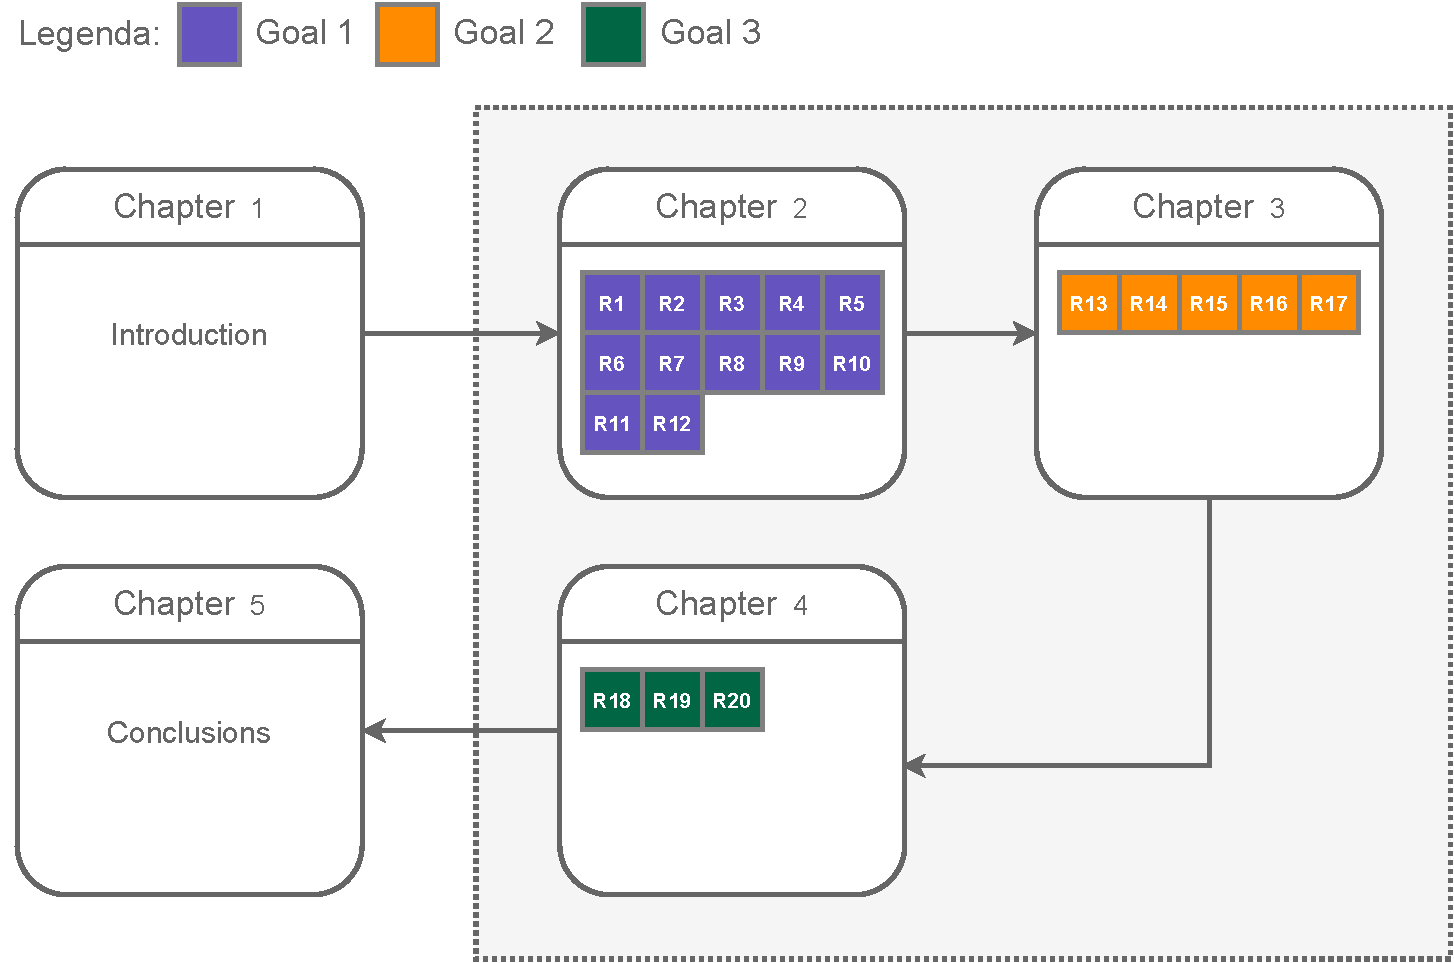
\includegraphics[width=.9\textwidth]{figures/thesis-organization.pdf}
	\end{figure}
\end{frame}

%%%%%%%%%%%%%%%%%%%%%%%%%%%%%%%%%%%%
%%%%%%%%%%%%%%%%%%%%%%%%%%%%%%%%%%%%

\bgroup
\begin{frame}[plain, c]{}
    \begin{center}
        \LARGE \colorbox{RoyalPurple}{\textcolor{White}{Goal 1}}:\\
        \Large Understand the \alert{state of the art} in bug \alert{severity level prediction} researching in FLOSS
    \end{center}
\end{frame}
\egroup

%%%%%%%%%%%%%%%%%%%%%%%%%%%%%%%%%%%%
%%%%%%%%%%%%%%%%%%%%%%%%%%%%%%%%%%%%
\subsection{Questions and Methodology}


%%%%%%%%%%%%%%%%%%%%%%%%%%%%%%%%%%%%
%%%%%%%%%%%%%%%%%%%%%%%%%%%%%%%%%%%%
\begin{frame}[t,fragile]{\colorbox{RoyalPurple}{\textcolor{White}{Goal 1}}:Research Questions}
    \begin{figure}
        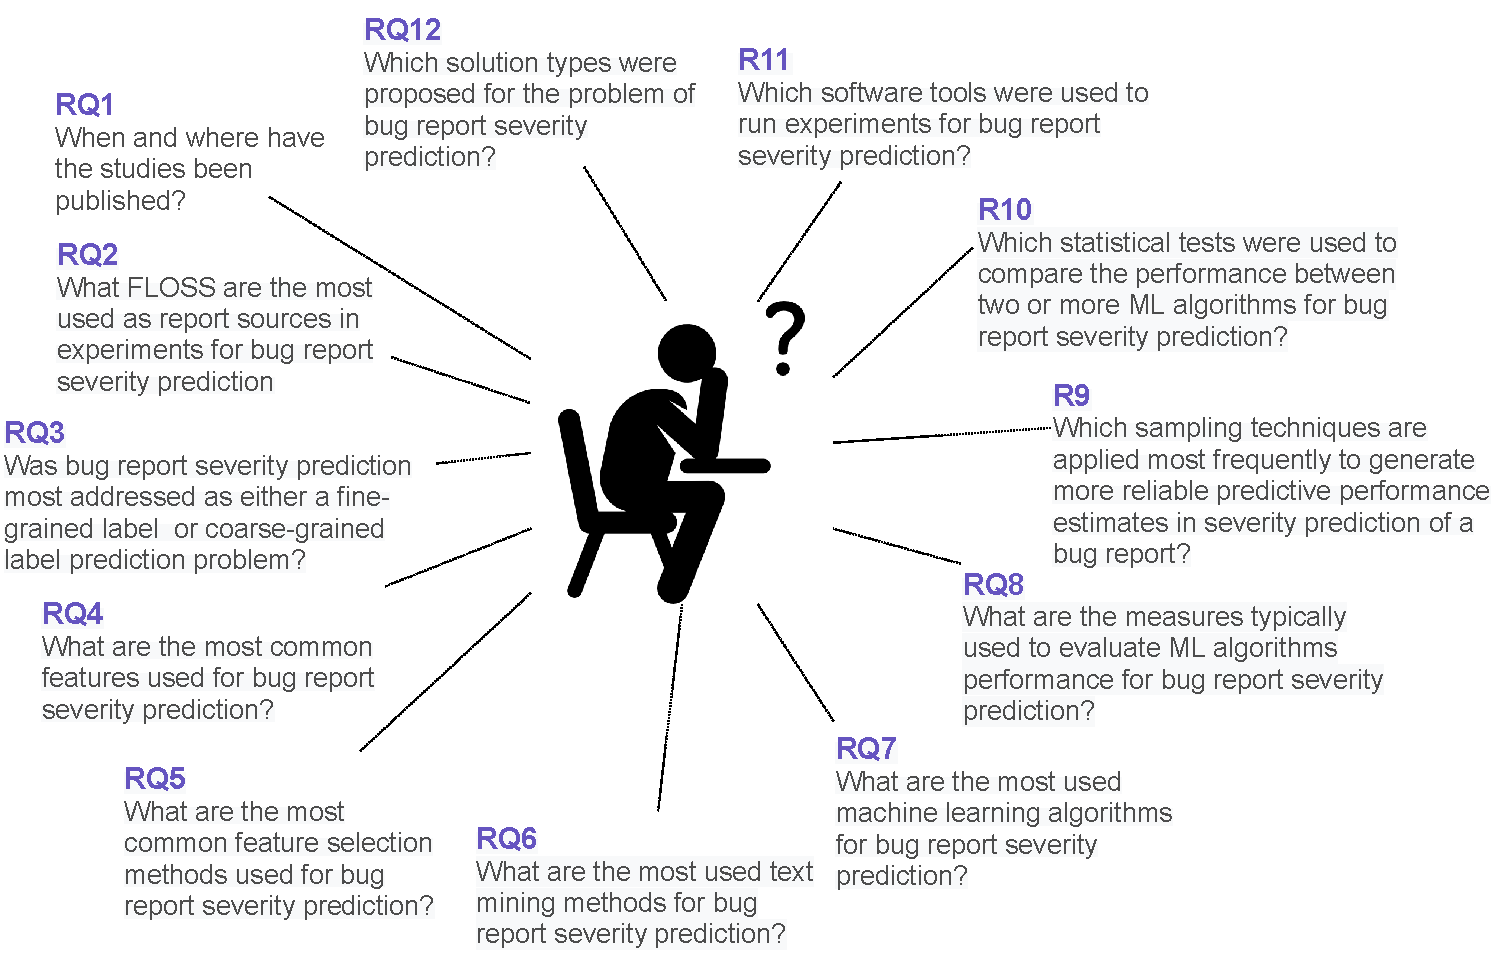
\includegraphics[width=\textwidth]{figures/goal-1-research-questions.pdf}
    \end{figure}
\end{frame}

%%%%%%%%%%%%%%%%%%%%%%%%%%%%%%%%%%%%
%%%%%%%%%%%%%%%%%%%%%%%%%%%%%%%%%%%%
\begin{frame}[t,fragile]{\colorbox{RoyalPurple}{\textcolor{White}{Goal 1}}:Research Methodology}
    \begin{figure}
        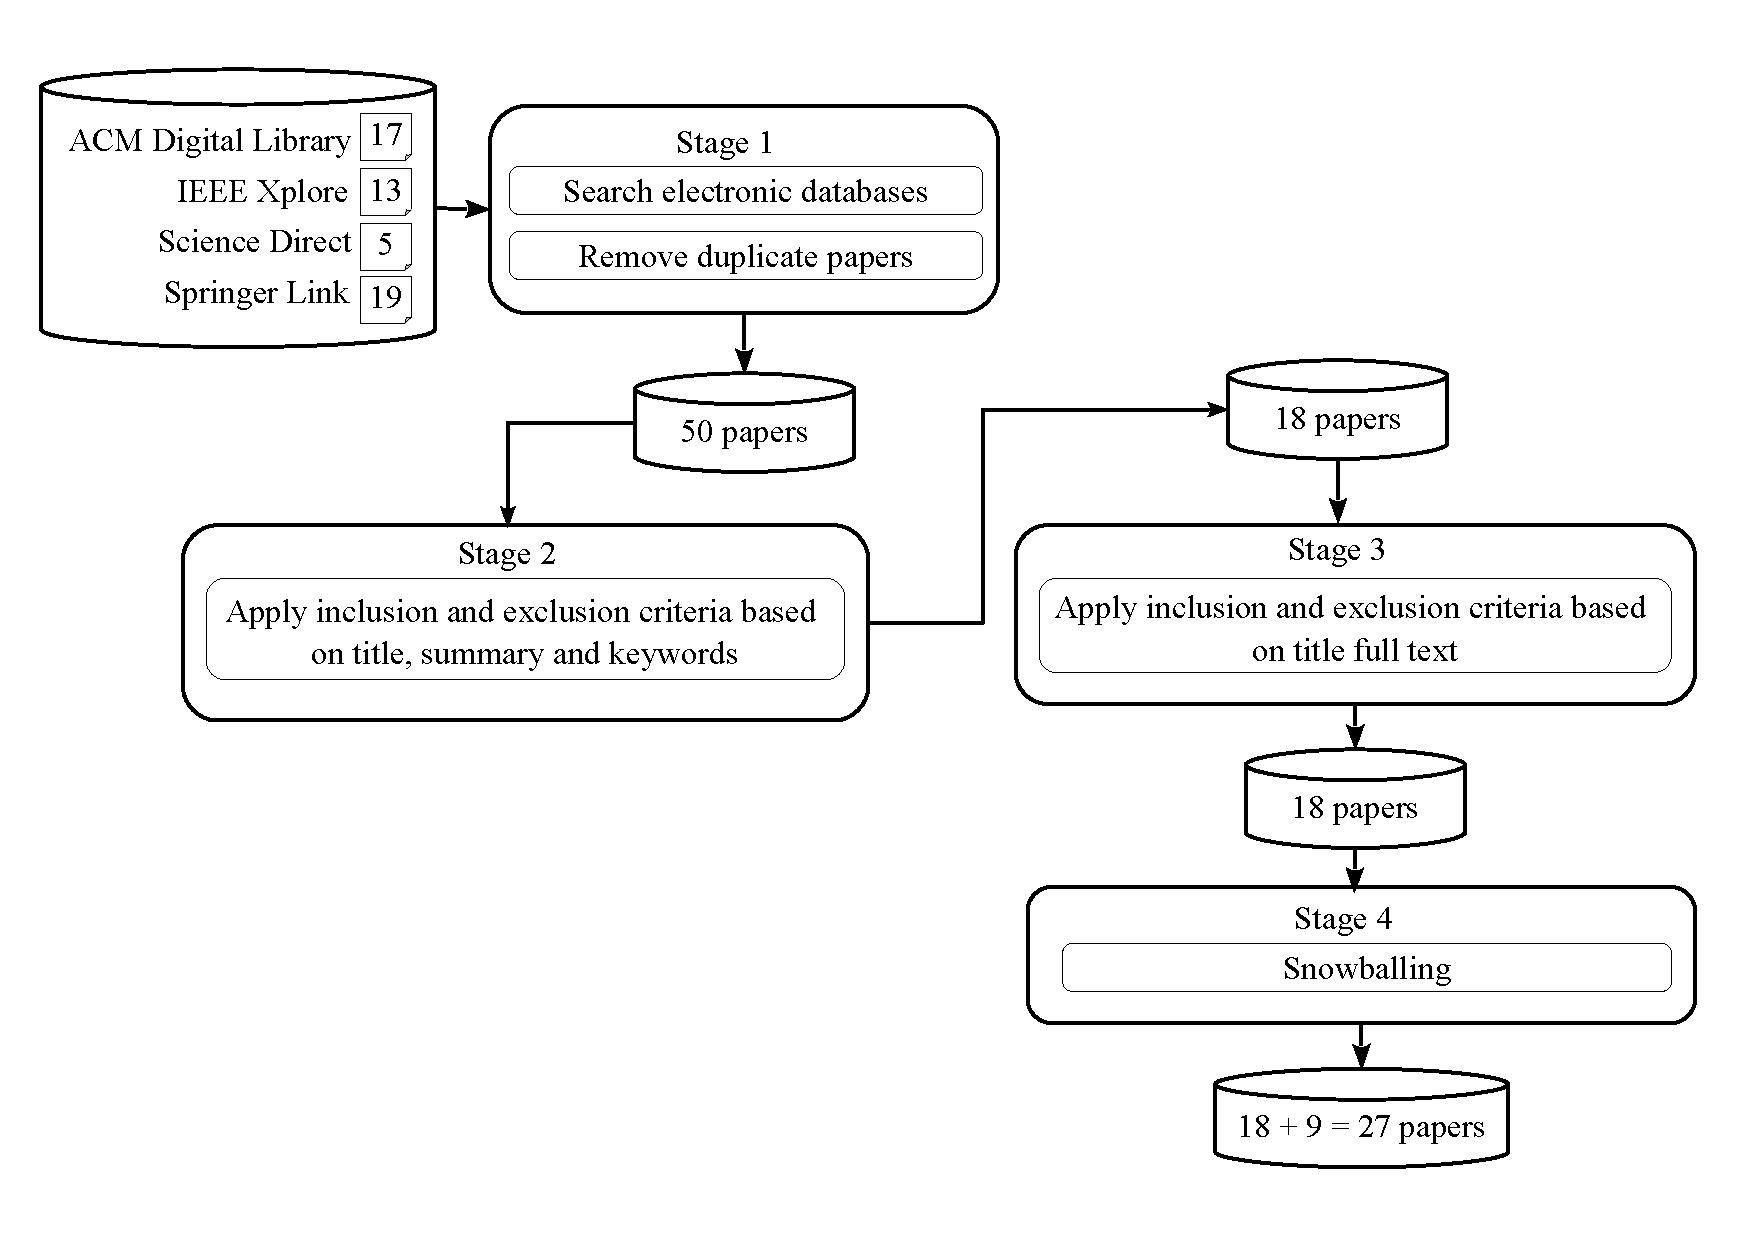
\includegraphics[width=.9\textwidth]{figures/goal-1-research-methodology.pdf}
    \end{figure}
\end{frame}

%%%%%%%%%%%%%%%%%%%%%%%%%%%%%%%%%%%%
%%%%%%%%%%%%%%%%%%%%%%%%%%%%%%%%%%%%
\subsection{Results and Discussions}

%%%%%%%%%%%%%%%%%%%%%%%%%%%%%%%%%%%%
%%%%%%%%%%%%%%%%%%%%%%%%%%%%%%%%%%%%
\begin{frame}[t,fragile]{\colorbox{RoyalPurple}{\textcolor{White}{Goal 1}}:Results and Discussions}
	\begin{center}
		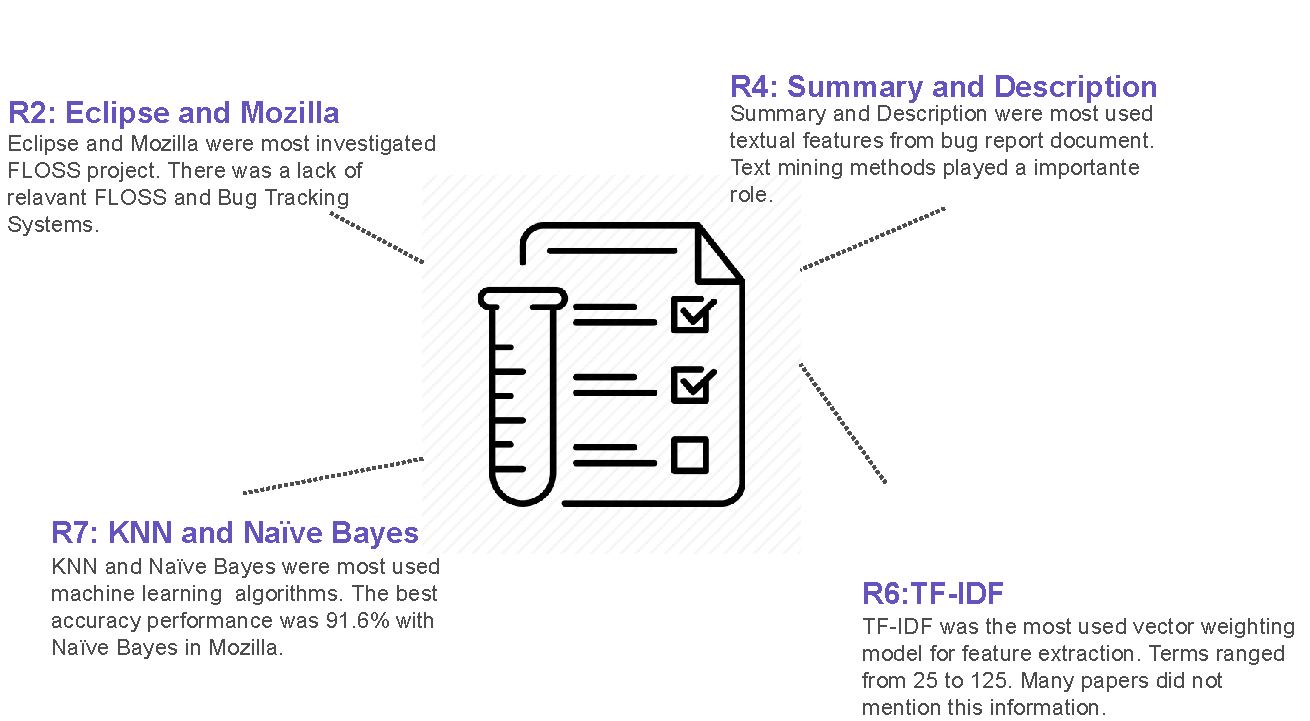
\includegraphics[width=\textwidth]{figures/goal-1-research-results.pdf}
	\end{center}
\end{frame}

%%%%%%%%%%%%%%%%%%%%%%%%%%%%%%%%%%%%
%%%%%%%%%%%%%%%%%%%%%%%%%%%%%%%%%%%%
\begin{frame}[t,fragile]{\colorbox{RoyalPurple}{\textcolor{White}{Goal 1}}:Results and Discussions}
	\begin{center}
		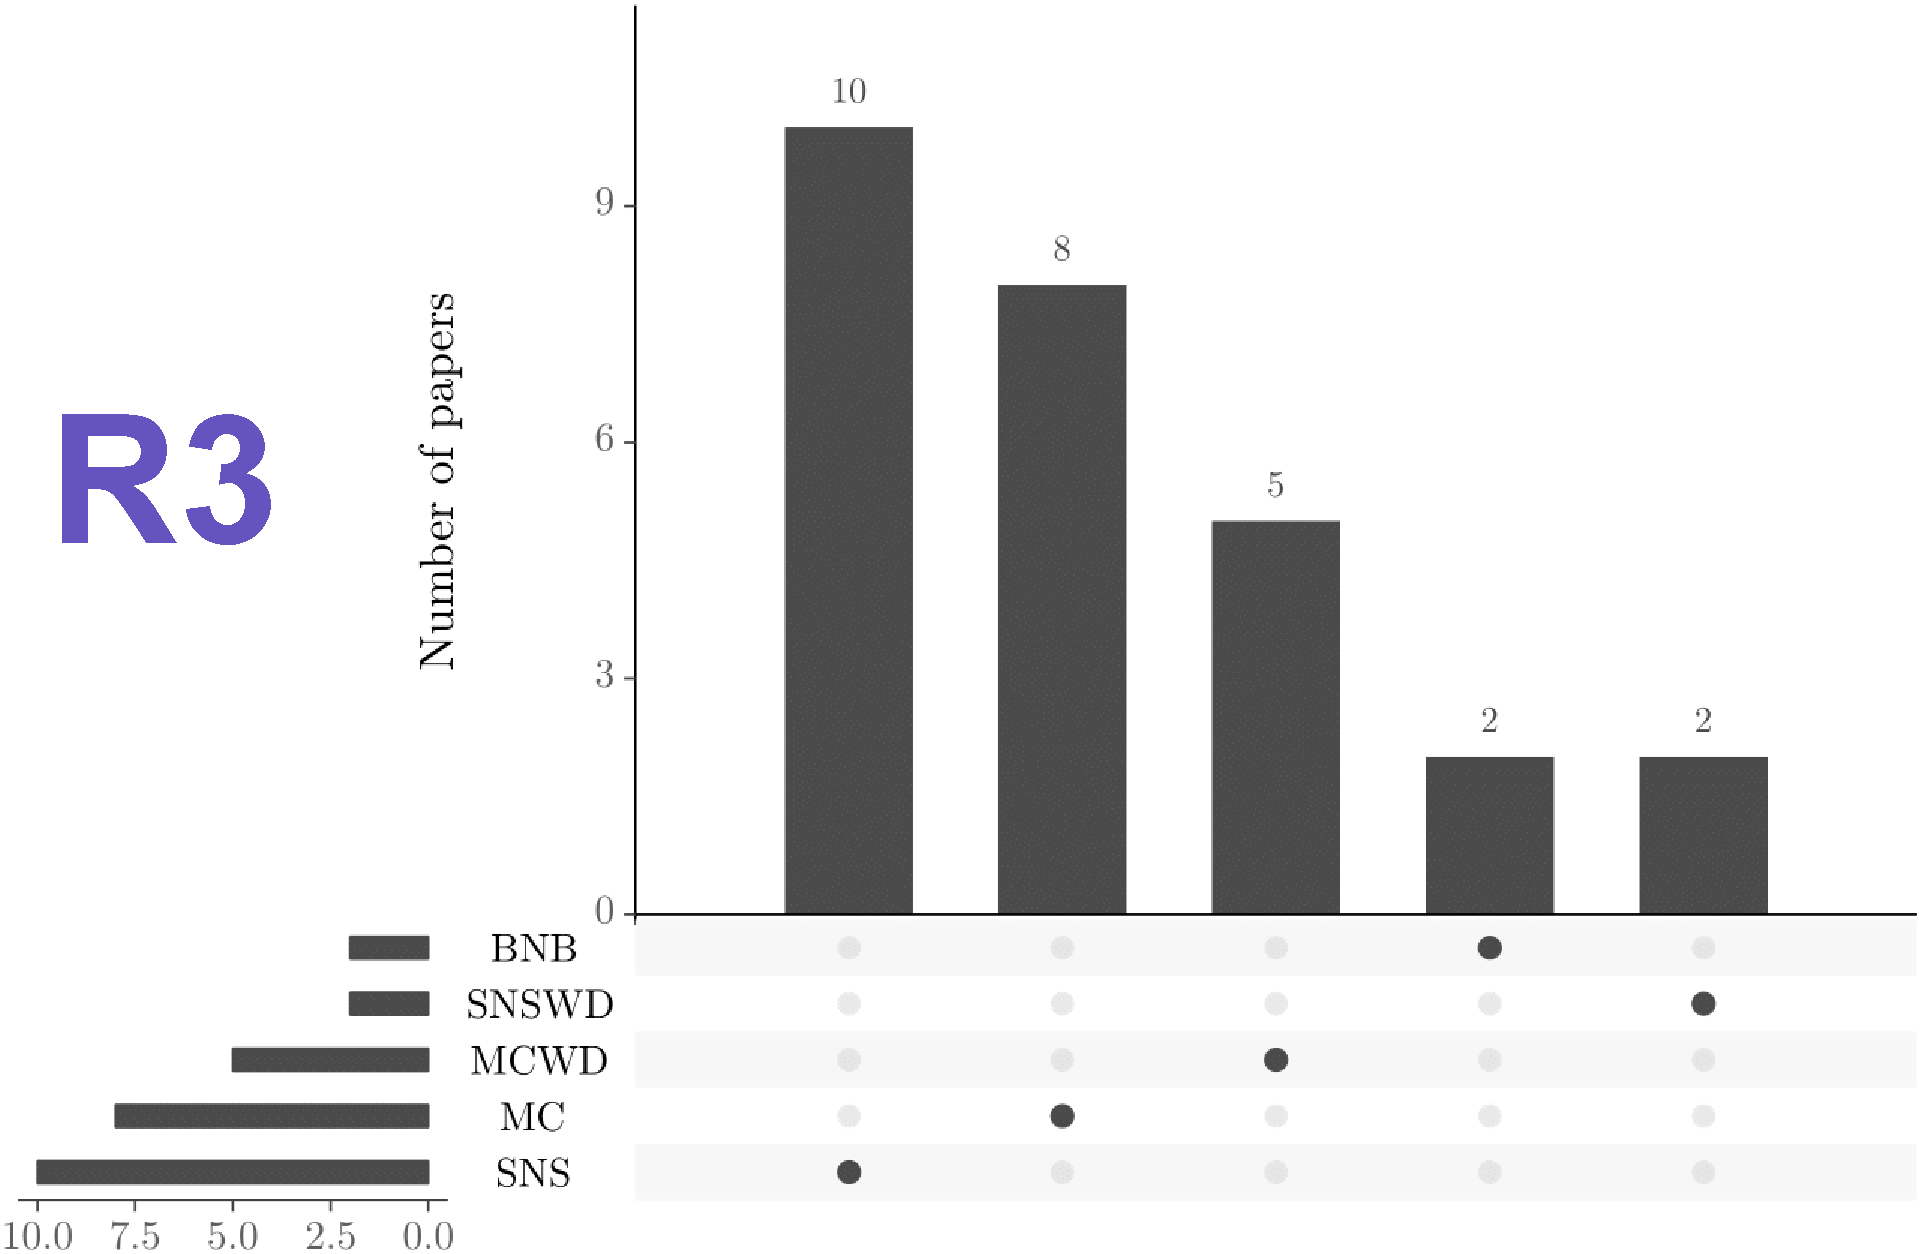
\includegraphics[width=.9\textwidth]{figures/distribution-by-problem-category-in-ups.pdf}
	\end{center}
\end{frame}

%%%%%%%%%%%%%%%%%%%%%%%%%%%%%%%%%%%%
%%%%%%%%%%%%%%%%%%%%%%%%%%%%%%%%%%%%
\subsection{Lessons Learned and Contributions}

%%%%%%%%%%%%%%%%%%%%%%%%%%%%%%%%%%%%
%%%%%%%%%%%%%%%%%%%%%%%%%%%%%%%%%%%%
\begin{frame}[t,fragile]{\colorbox{RoyalPurple}{\textcolor{White}{Goal 1}}:Lessons Learned}
	\begin{itemize}
        \item Lack of investigation of other relevant FLOSS and BTS such as, \alert{Linux Kernel} and \alert{Github}
        \item New efforts to handle \alert{``normal"} severity are necessary
        \item Recent text mining or data-driven feature engineering methods may likely \alert{improve} outcomes
        \item Opportunity for investigating \alert{state-of-the-art} ML and DL algorithms
        \item Opportunity for investigating the \alert{impact} of the temporal evolution of a bug report information in prediction problems
	\end{itemize}
\end{frame}

%%%%%%%%%%%%%%%%%%%%%%%%%%%%%%%%%%%%
%%%%%%%%%%%%%%%%%%%%%%%%%%%%%%%%%%%%
\begin{frame}[t,fragile]{\colorbox{RoyalPurple}{\textcolor{White}{Goal 1}}:Contributions}
	\begin{itemize}
		\item Categorization scheme to \alert{organize} the experiments 
		\item \alert{Challenges}, \alert{open issues}, and \alert{future directions}
	\end{itemize}
\end{frame}

%%%%%%%%%%%%%%%%%%%%%%%%%%%%%%%%%%%%
%%%%%%%%%%%%%%%%%%%%%%%%%%%%%%%%%%%%
\bgroup
\begin{frame}[plain, c]{}
    \begin{center}
        \LARGE \colorbox{BurntOrange}{\textcolor{White}{Goal 2}}\\
        \Large Compare traditional ML algorithms in \alert{long-lived bug prediction} in FLOSS
    \end{center}
\end{frame}
\egroup

%%%%%%%%%%%%%%%%%%%%%%%%%%%%%%%%%%%%
%%%%%%%%%%%%%%%%%%%%%%%%%%%%%%%%%%%%
\begin{frame}[t,fragile]{\colorbox{BurntOrange}{\textcolor{White}{Goal 2}}:Research Questions}
    \begin{figure}
        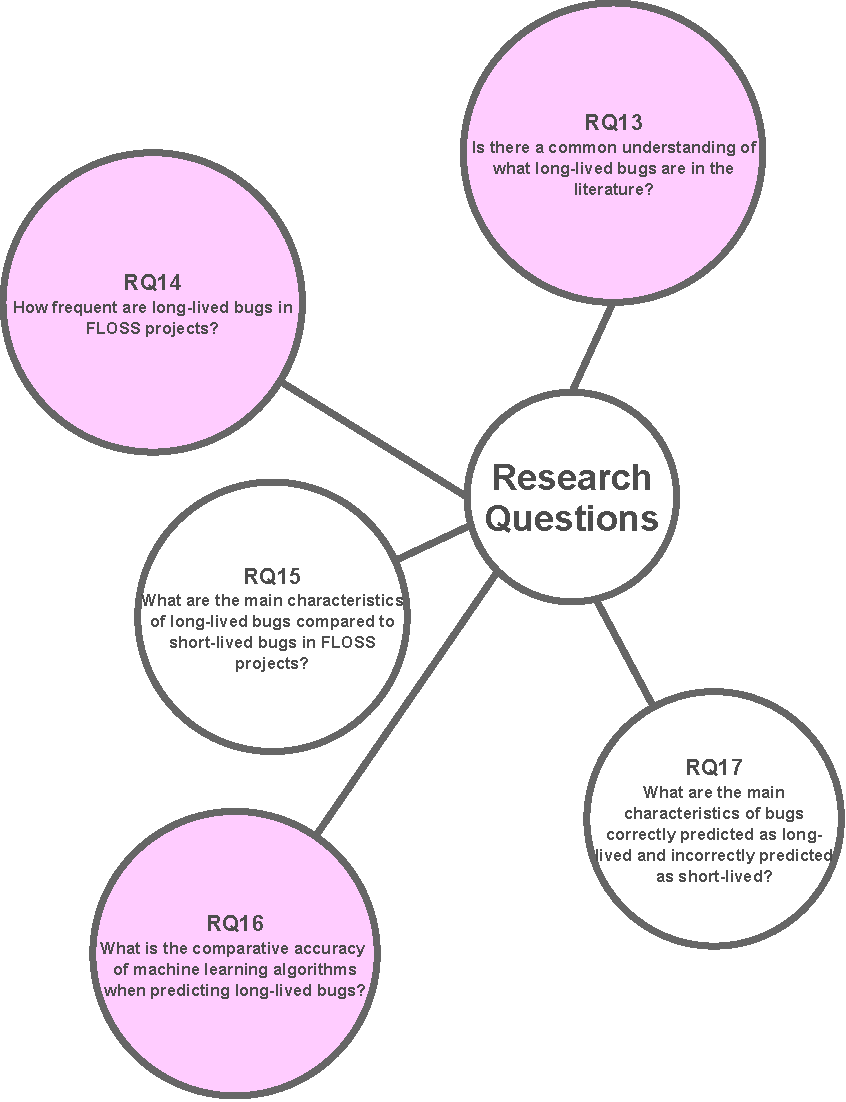
\includegraphics[width=.9\textwidth]{figures/goal-2-research-questions.pdf}
    \end{figure}
\end{frame}

%%%%%%%%%%%%%%%%%%%%%%%%%%%%%%%%%%%%
%%%%%%%%%%%%%%%%%%%%%%%%%%%%%%%%%%%%
\begin{frame}[t,fragile]{\colorbox{BurntOrange}{\textcolor{White}{Goal 2}}:Research Methodology}
    \begin{figure}
        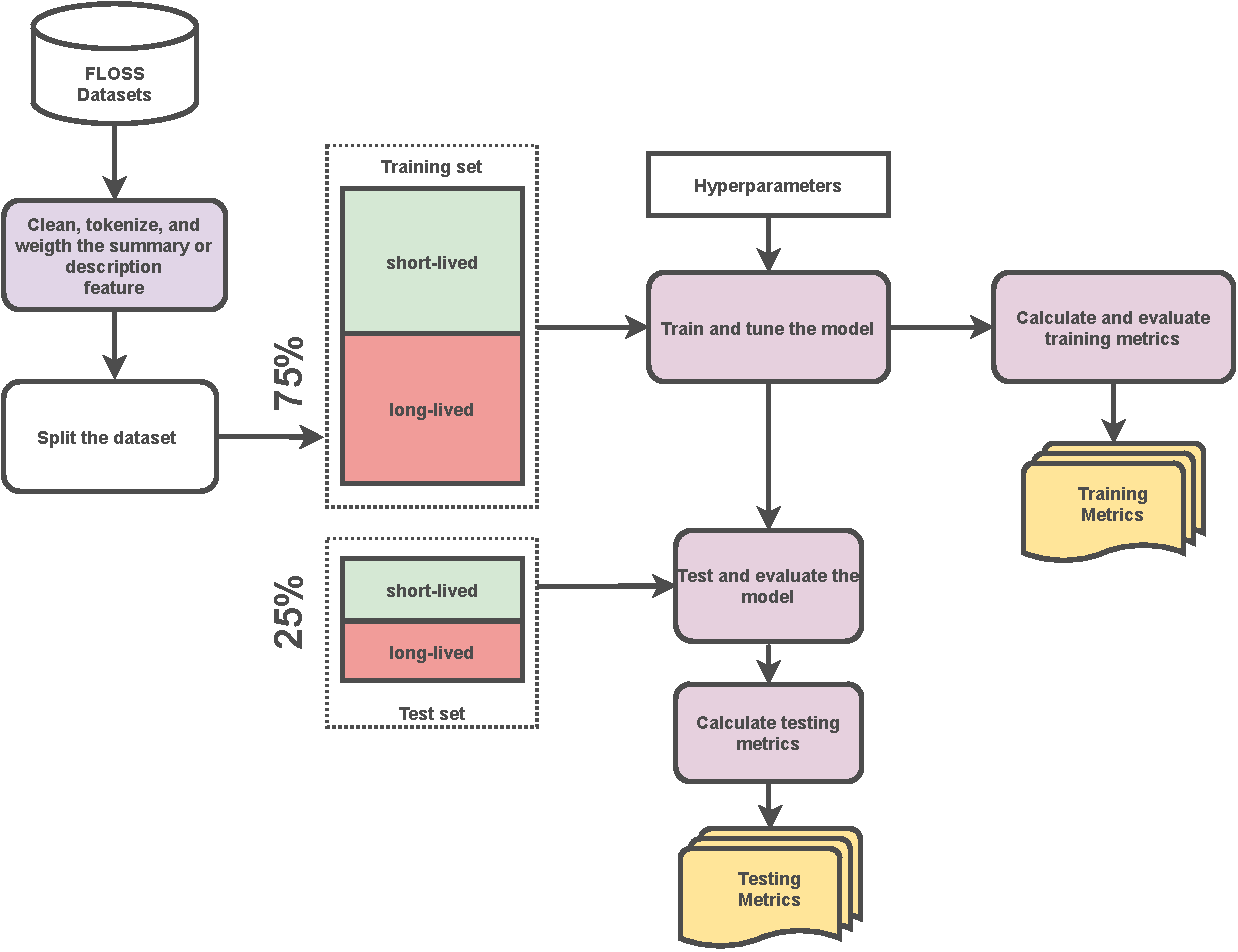
\includegraphics[width=.8\textwidth]{figures/goal-2-research-methodology-3.pdf}
    \end{figure}
\end{frame}

%%%%%%%%%%%%%%%%%%%%%%%%%%%%%%%%%%%%
%%%%%%%%%%%%%%%%%%%%%%%%%%%%%%%%%%%%
%\subsection{Experimental Setup}
\begin{frame}[c	,fragile]{\colorbox{BurntOrange}{\textcolor{White}{Goal 2}}:Experimental Setup}
	\begin{figure}
		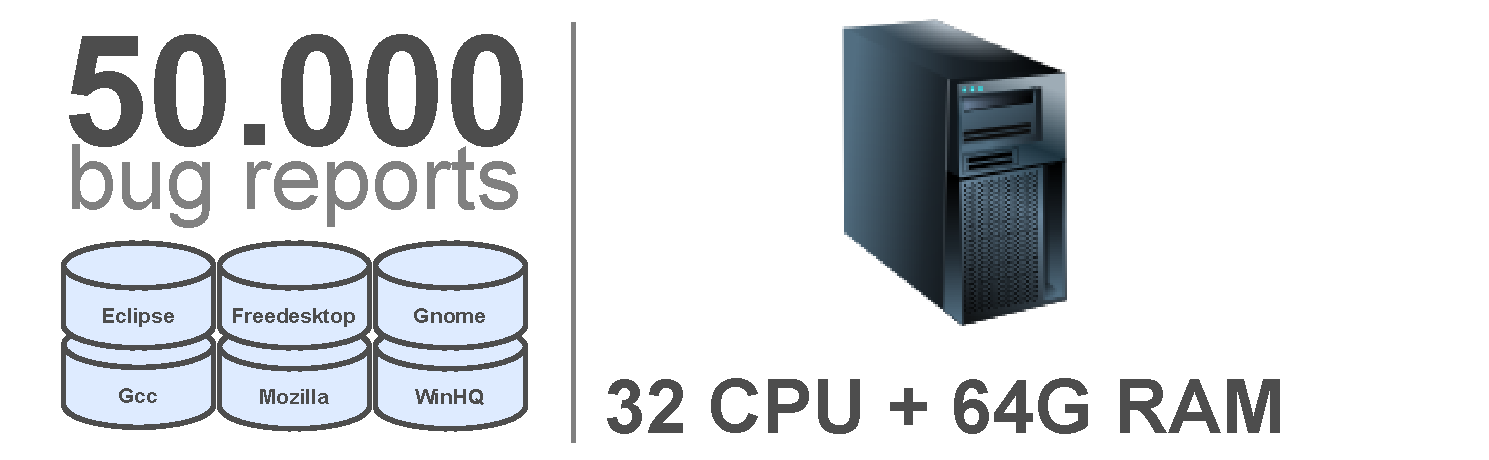
\includegraphics[width=\textwidth]{figures/experimental-setup-1.pdf}
	\end{figure}
\end{frame}


%%%%%%%%%%%%%%%%%%%%%%%%%%%%%%%%%%%%
%%%%%%%%%%%%%%%%%%%%%%%%%%%%%%%%%%%%
\begin{frame}[t,fragile]{\colorbox{BurntOrange}{\textcolor{White}{Goal 2}}:Results and Discussions}
	\begin{figure}
		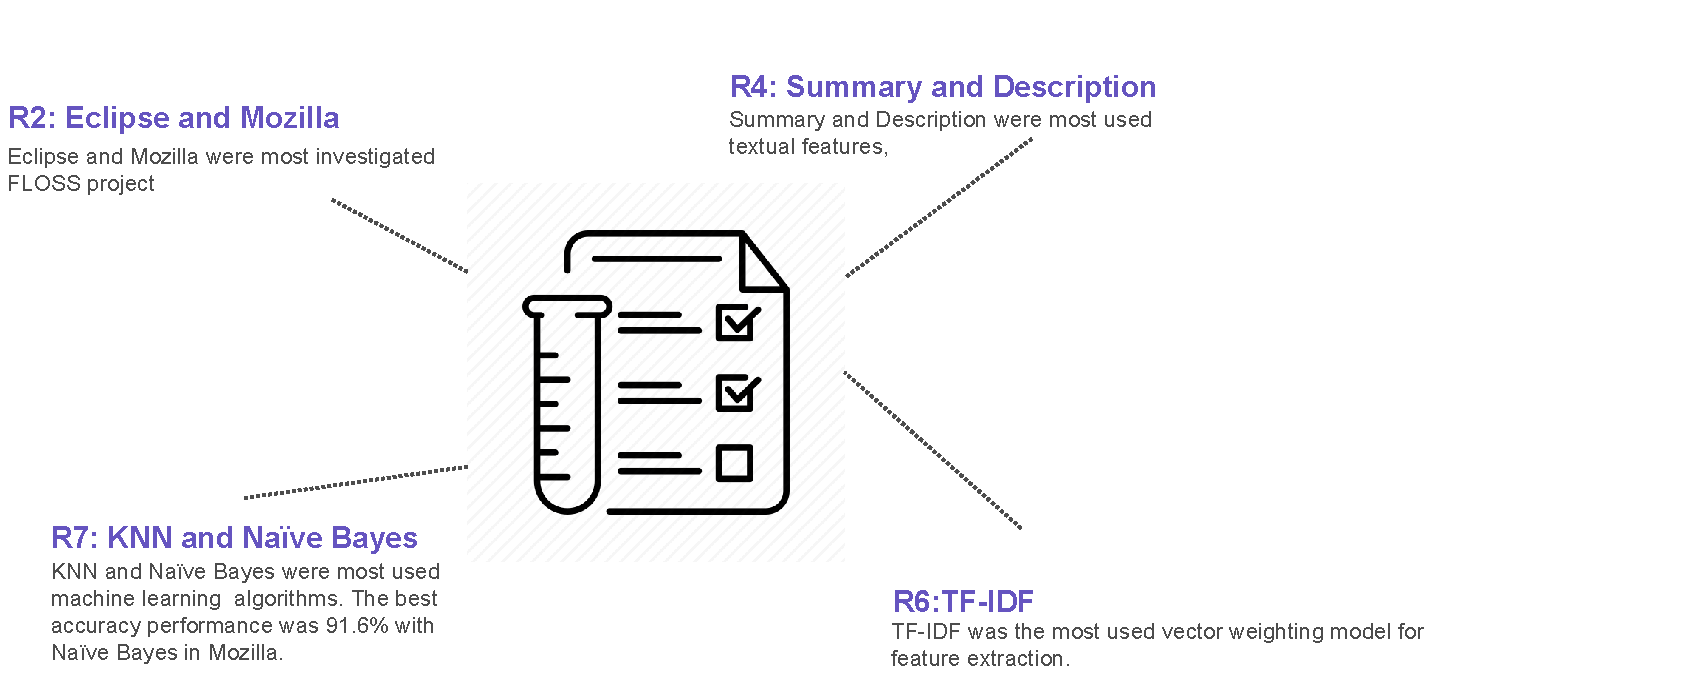
\includegraphics[width=\textwidth]{figures/goal-2-research-results.pdf}
	\end{figure}
\end{frame}

%%%%%%%%%%%%%%%%%%%%%%%%%%%%%%%%%%%%
%%%%%%%%%%%%%%%%%%%%%%%%%%%%%%%%%%%%
\begin{frame}[t,fragile]{\colorbox{BurntOrange}{\textcolor{White}{Goal 2}}:Results and Discussions}
	\begin{figure}
		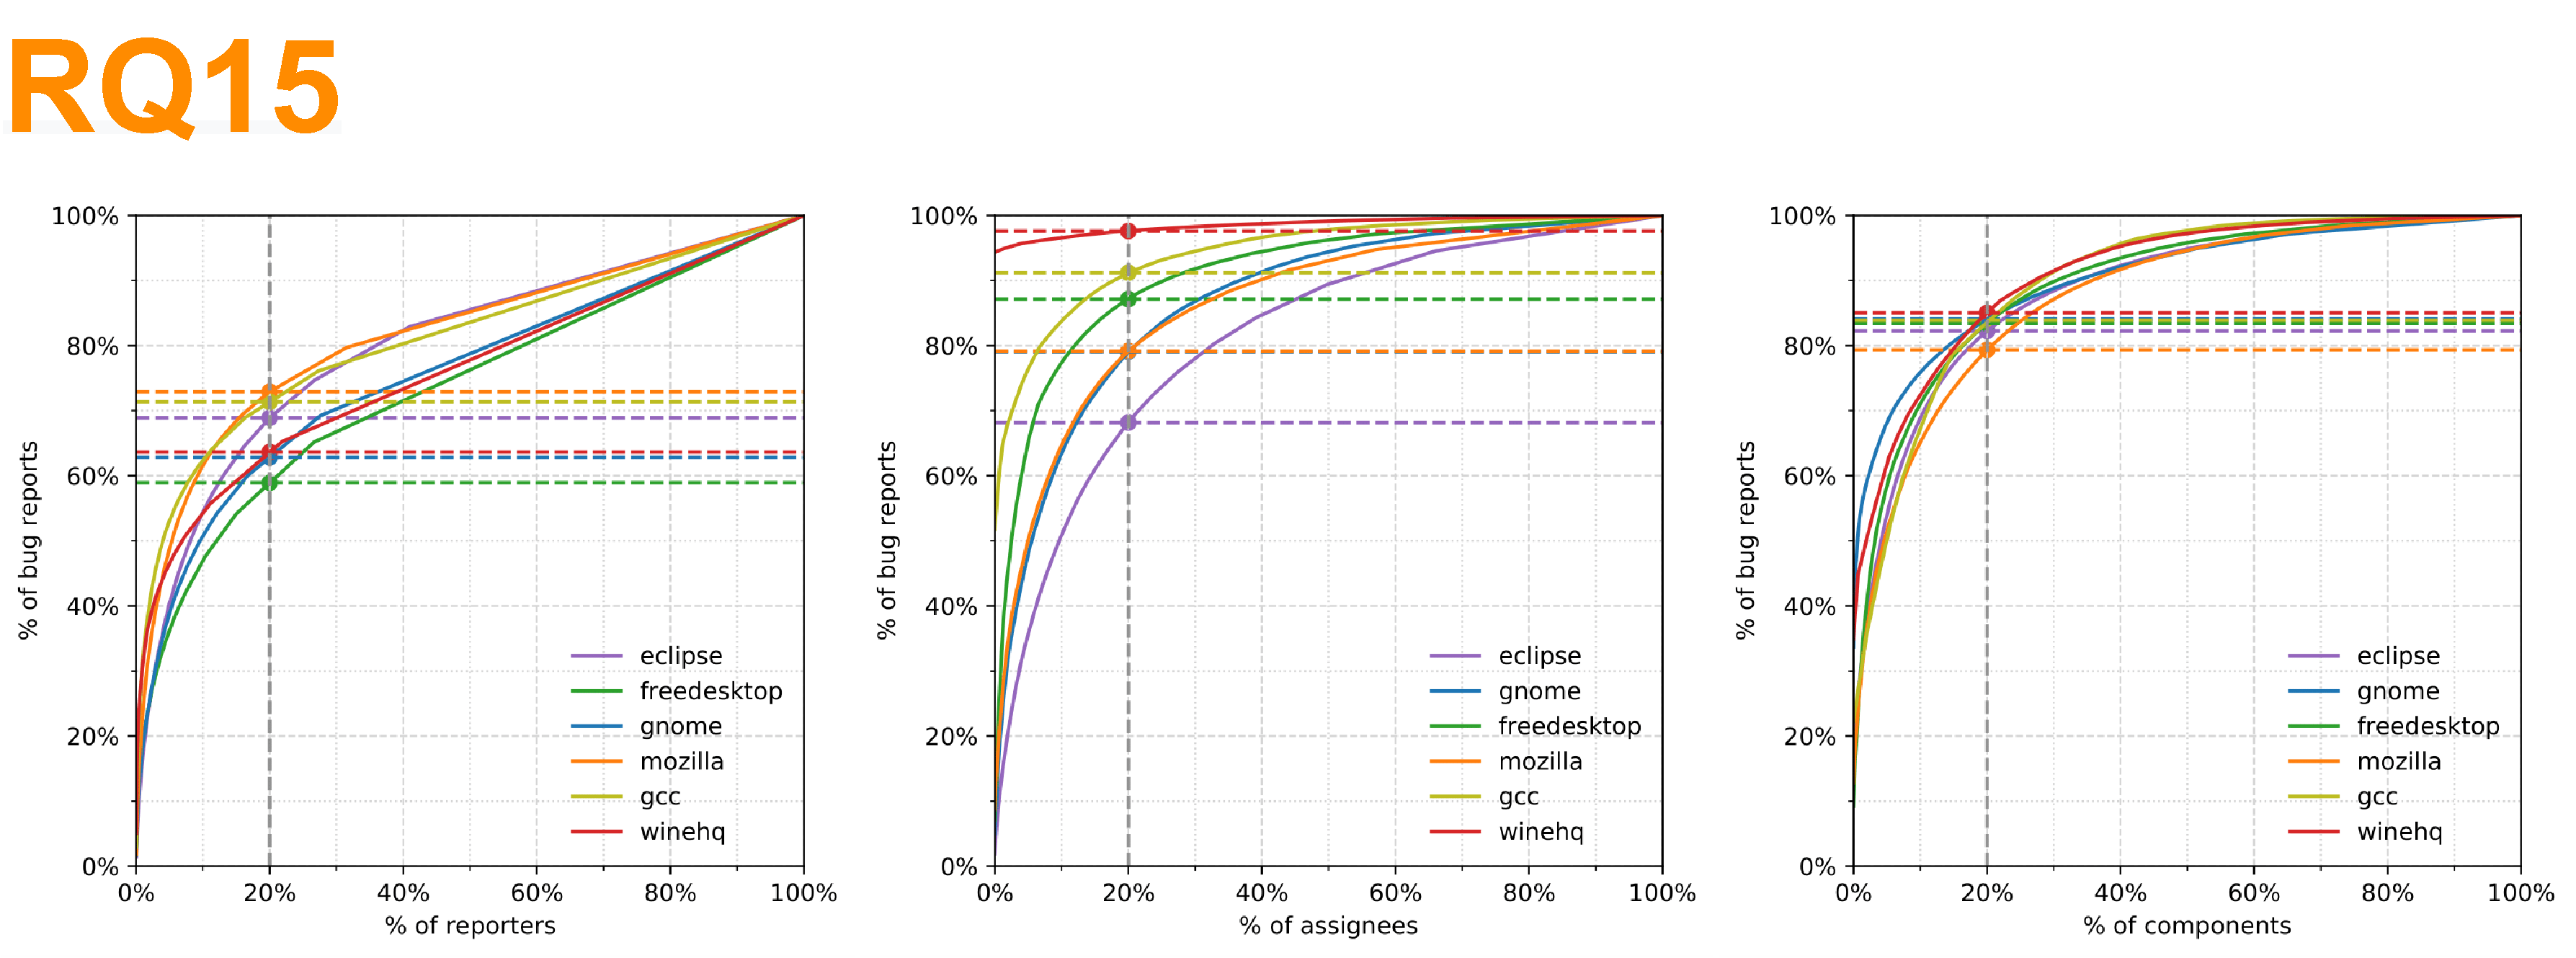
\includegraphics[width=\textwidth]{figures/r15_reporters_assignees_components.pdf}
	\end{figure}
\end{frame}

%%%%%%%%%%%%%%%%%%%%%%%%%%%%%%%%%%%%
%%%%%%%%%%%%%%%%%%%%%%%%%%%%%%%%%%%%
\begin{frame}[t,fragile]{\colorbox{BurntOrange}{\textcolor{White}{Goal 2}}:Lessons Learned}
	\begin{itemize}
		\item \alert{Relevant} percentage of long-lived bugs	  
		\item \alert{Differences} between short-lived population and long-lived population
		\item \alert{Shortage} of resources in projects with the greatest number of long-lived bugs
	\end{itemize}
\end{frame}

%%%%%%%%%%%%%%%%%%%%%%%%%%%%%%%%%%%%
%%%%%%%%%%%%%%%%%%%%%%%%%%%%%%%%%%%%
\begin{frame}[t,fragile]{\colorbox{BurntOrange}{\textcolor{White}{Goal 2}}:Contributions}
	\begin{itemize}
		\item \alert{Characterization} of long-lived bugs in FLOSS
		\item Evaluation of the \alert{performance} of machine learning algorithms
	\end{itemize}
\end{frame}

%%%%%%%%%%%%%%%%%%%%%%%%%%%%%%%%%%%%
%%%%%%%%%%%%%%%%%%%%%%%%%%%%%%%%%%%%
\bgroup
\begin{frame}[plain, c]{}
    \begin{center}
        \LARGE \colorbox{OliveGreen}{\textcolor{White}{Goal 3}}\\
        \Large Evaluate \alert{BERT-based feature extraction} in long-lived bug prediction in FLOSS
    \end{center}
\end{frame}
\egroup

%%%%%%%%%%%%%%%%%%%%%%%%%%%%%%%%%%%%
%%%%%%%%%%%%%%%%%%%%%%%%%%%%%%%%%%%%
\begin{frame}[t,fragile]{\alert{B}idirectional \alert{E}ncoder \alert{R}epresentation from \alert{T}ransformers}
	\begin{figure}
		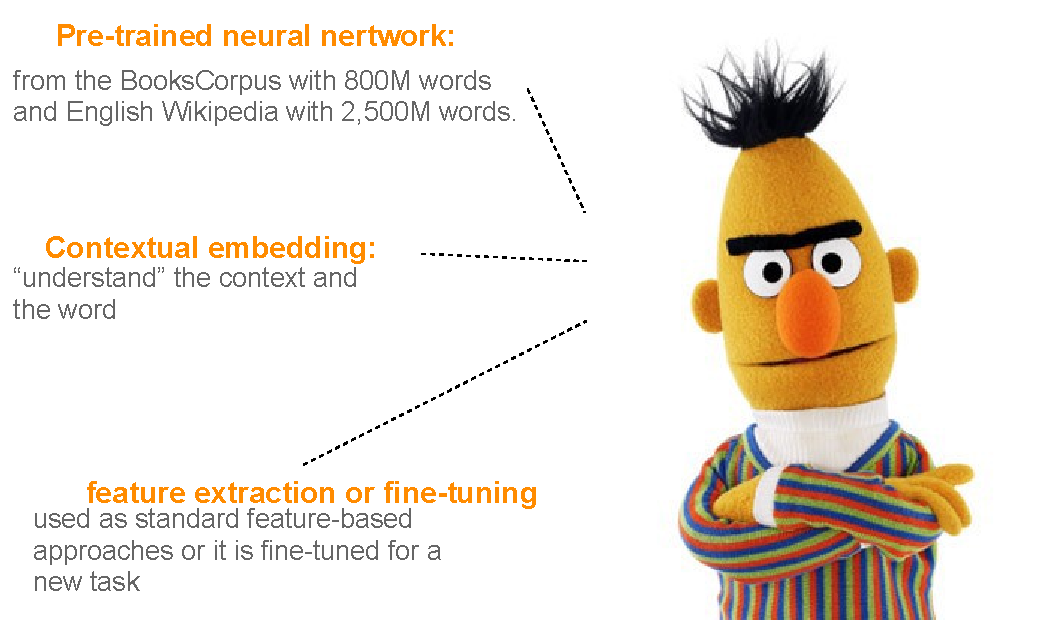
\includegraphics[width=.70\textwidth]{figures/bert-summary.pdf}
	\end{figure}
\end{frame}

%%%%%%%%%%%%%%%%%%%%%%%%%%%%%%%%%%%%
%%%%%%%%%%%%%%%%%%%%%%%%%%%%%%%%%%%%
\begin{frame}[t,fragile]{\colorbox{OliveGreen}{\textcolor{White}{Goal 3}}:Research Questions}
    \begin{figure}
        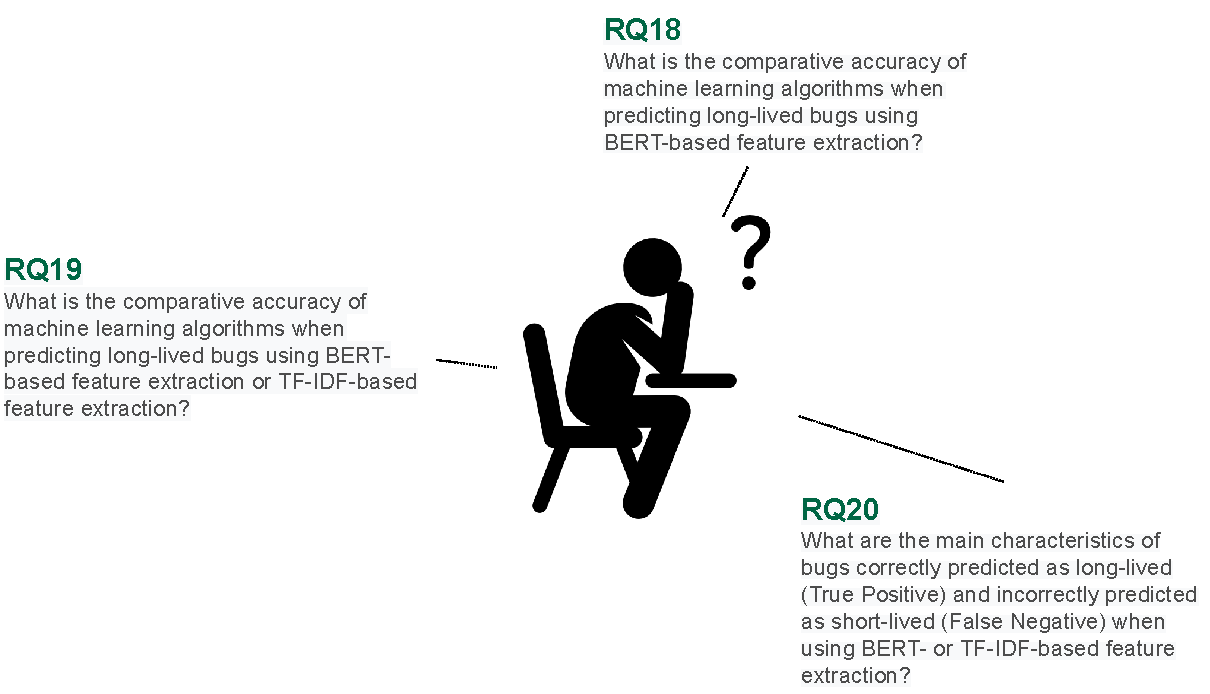
\includegraphics[width=.9\textwidth]{figures/goal-3-research-questions.pdf}
    \end{figure}
\end{frame}

%%%%%%%%%%%%%%%%%%%%%%%%%%%%%%%%%%%%
%%%%%%%%%%%%%%%%%%%%%%%%%%%%%%%%%%%%
\begin{frame}[t,fragile]{\colorbox{OliveGreen}{\textcolor{White}{Goal 3}}:Research Methodology}
	\begin{figure}
		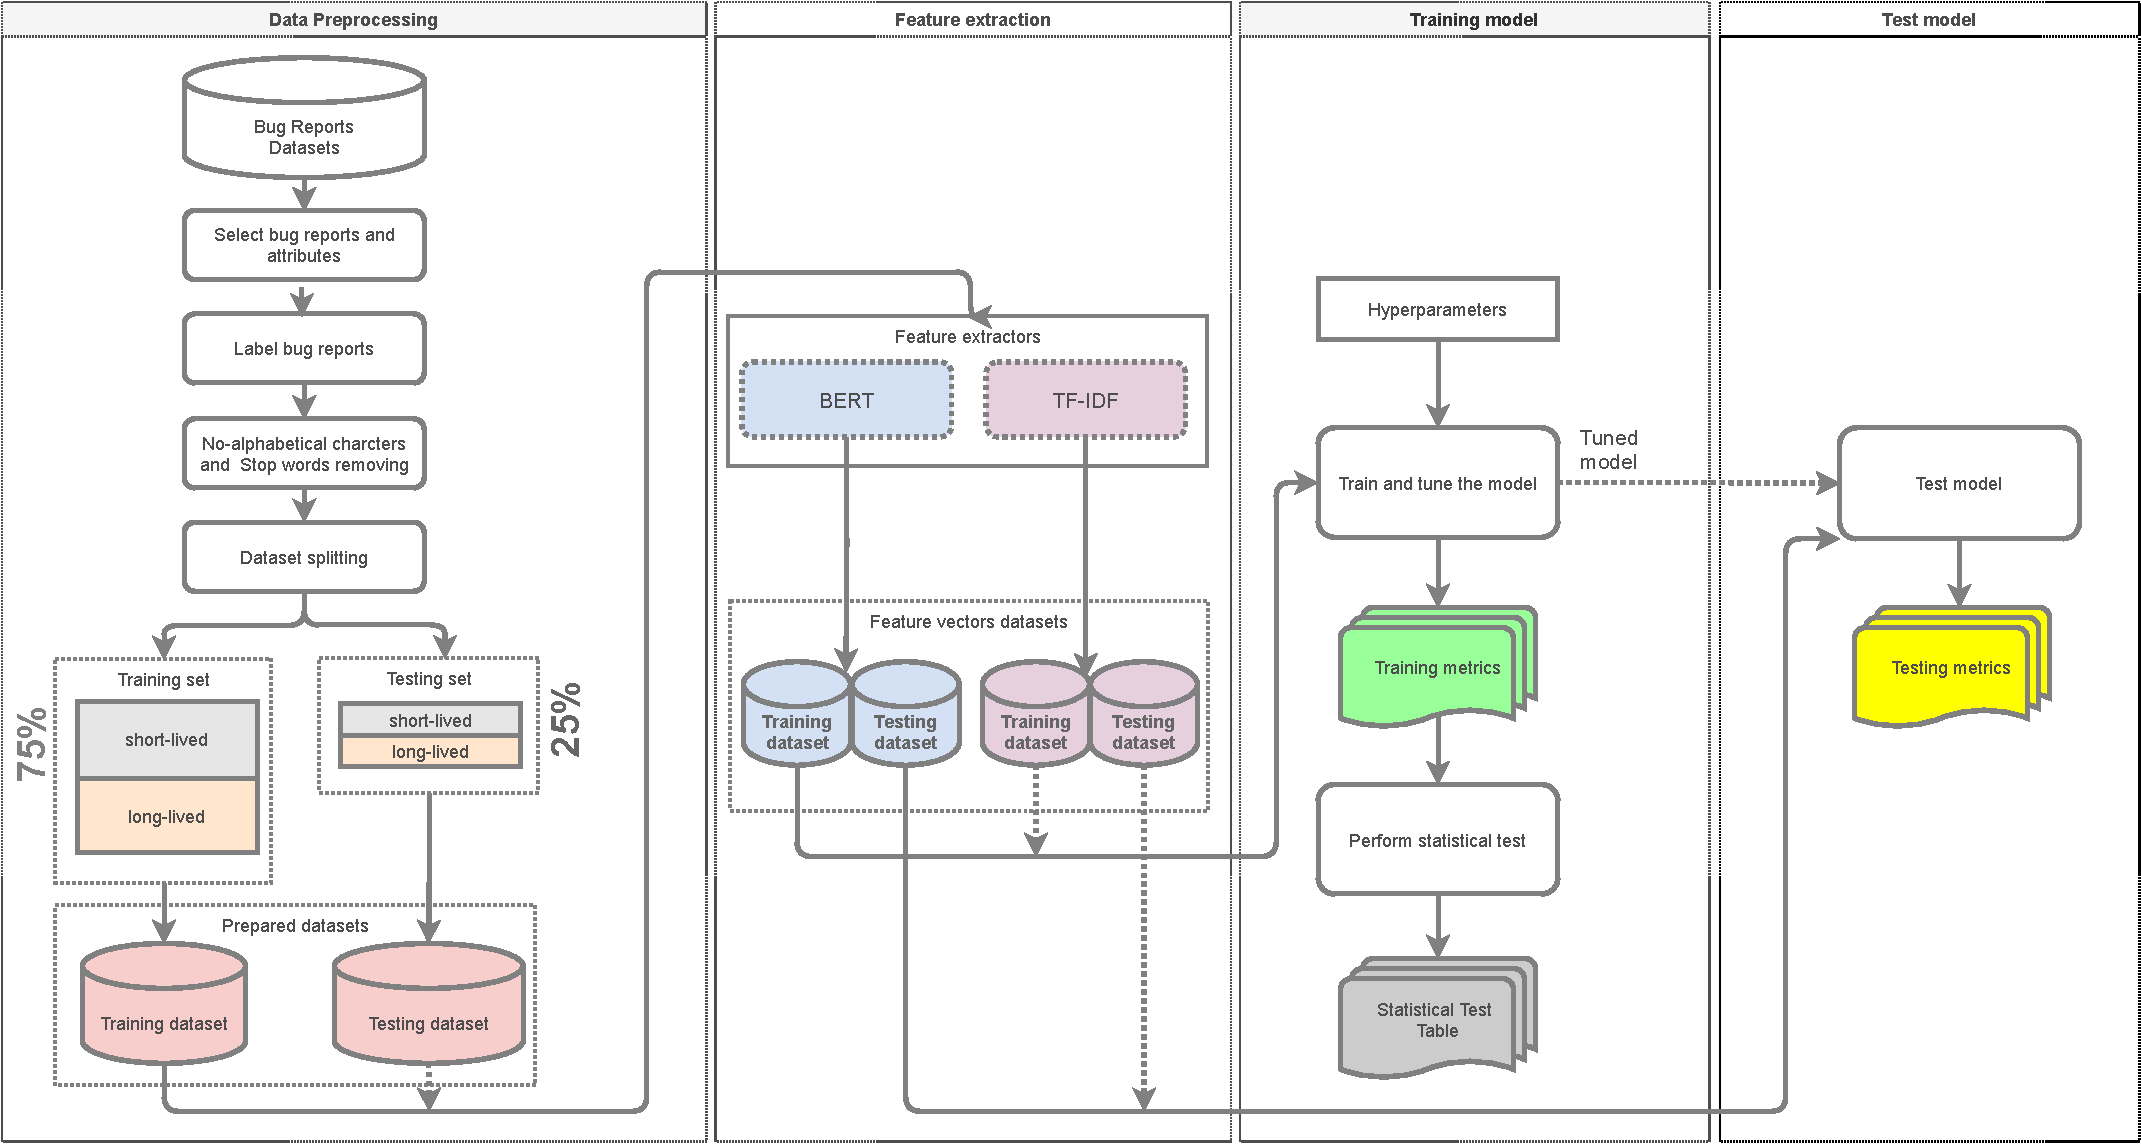
\includegraphics[width=\textwidth]{figures/goal-3-research-methodology.pdf}
	\end{figure}
\end{frame}

%%%%%%%%%%%%%%%%%%%%%%%%%%%%%%%%%%%%
%%%%%%%%%%%%%%%%%%%%%%%%%%%%%%%%%%%%
\begin{frame}[t,fragile]{\colorbox{OliveGreen}{\textcolor{White}{Goal 3}}:Results and Discussions}
	\begin{figure}
		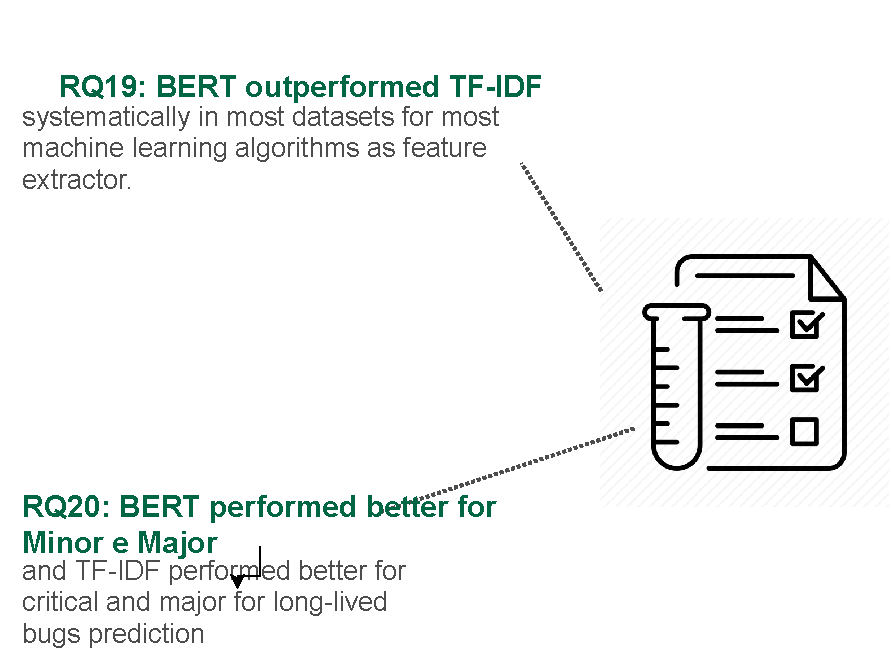
\includegraphics[width=.8\textwidth]{figures/goal-3-research-results.pdf}
	\end{figure}
\end{frame}

%%%%%%%%%%%%%%%%%%%%%%%%%%%%%%%%%%%%
%%%%%%%%%%%%%%%%%%%%%%%%%%%%%%%%%%%%
\begin{frame}[t,fragile]{\colorbox{OliveGreen}{\textcolor{White}{Goal 3}}:Results and Discussions}
	\begin{figure}
		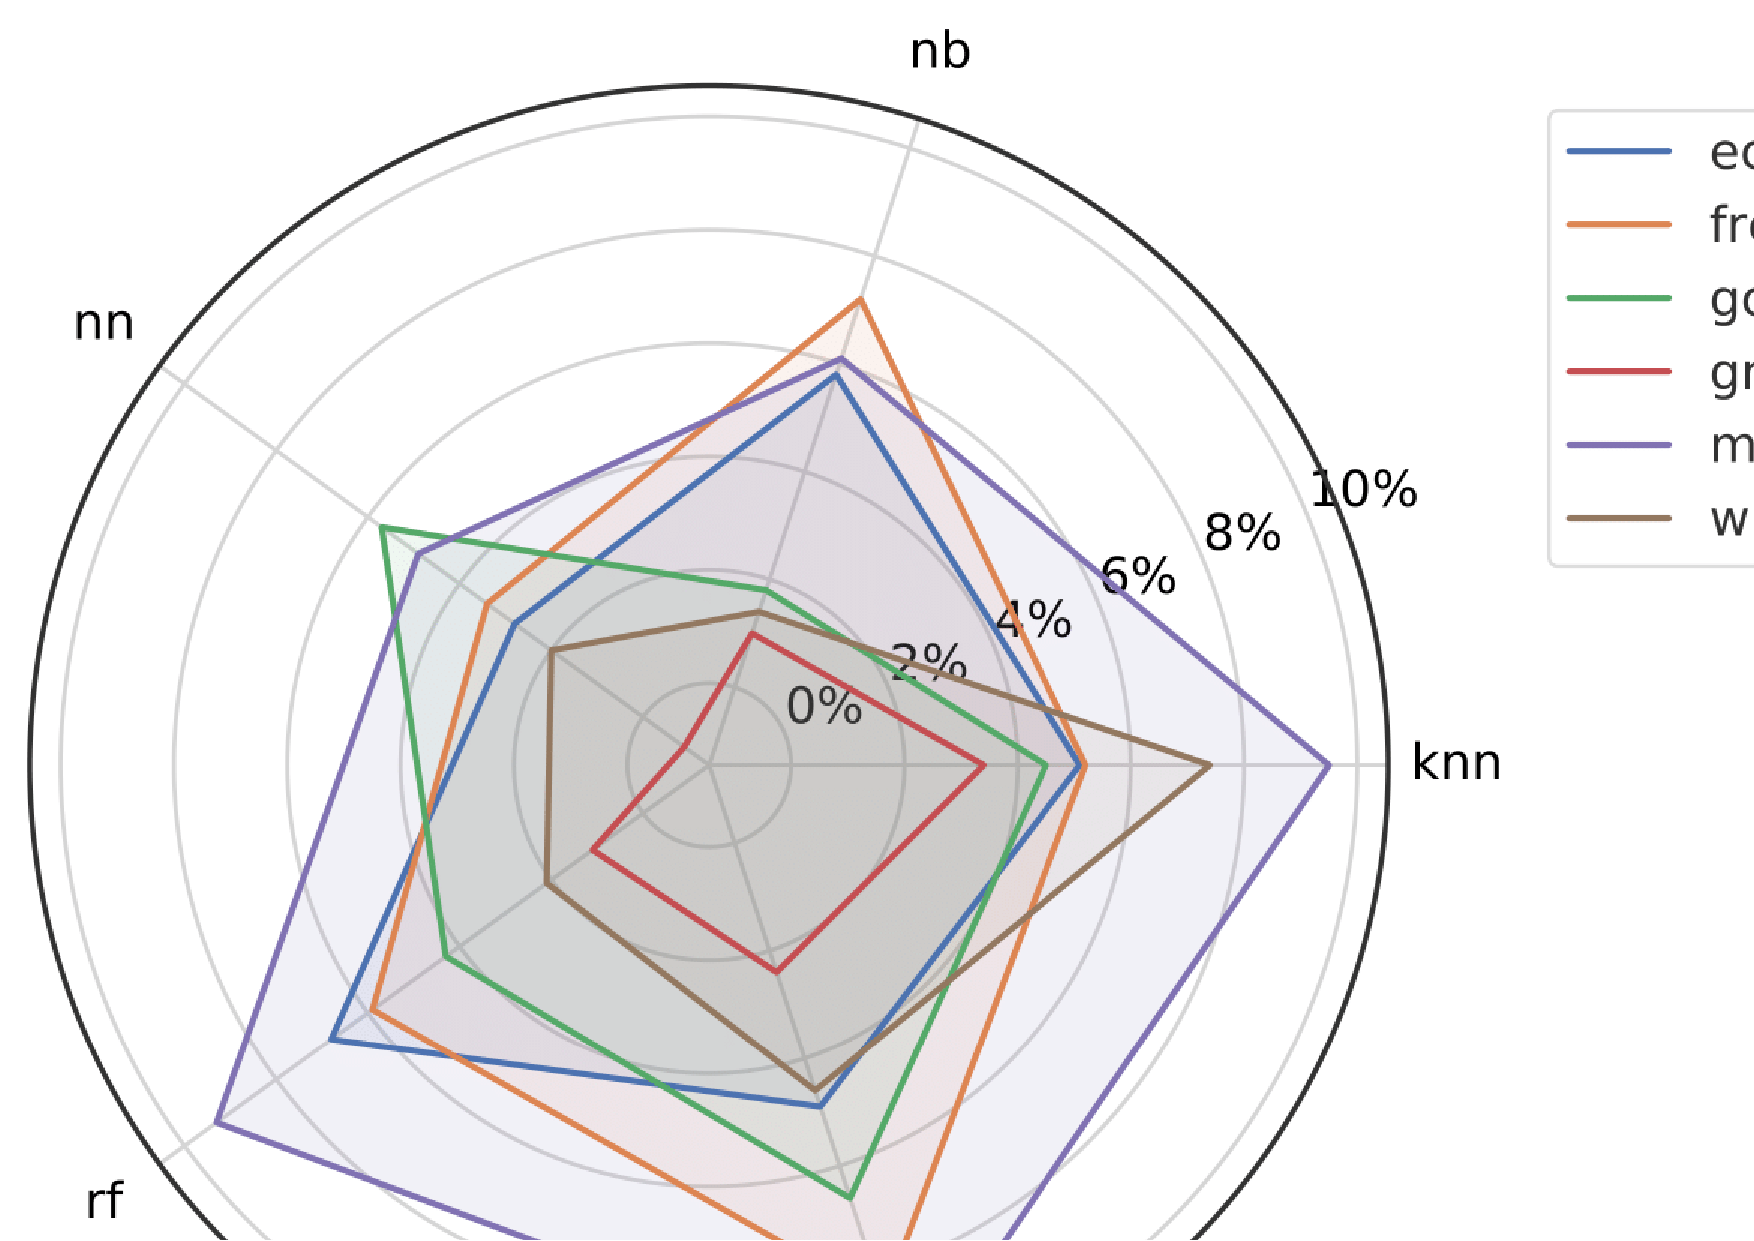
\includegraphics[width=.7\textwidth]{figures/goal-3-rq19.pdf}
	\end{figure}
\end{frame}

%%%%%%%%%%%%%%%%%%%%%%%%%%%%%%%%%%%%
%%%%%%%%%%%%%%%%%%%%%%%%%%%%%%%%%%%%
\begin{frame}[t,fragile]{\colorbox{OliveGreen}{\textcolor{White}{Goal 3}}:Lessons Learned}
	\begin{itemize}		
		\item The accuracy of ML algorithms using BERT-based feature extraction was \alert{very promising} 
		\item We observed that the accuracy from some bug reports attributes' perspectives somewhat \alert{varied}
	\end{itemize}
\end{frame}

%%%%%%%%%%%%%%%%%%%%%%%%%%%%%%%%%%%%
%%%%%%%%%%%%%%%%%%%%%%%%%%%%%%%%%%%%
%\section{Contributions}

%%%%%%%%%%%%%%%%%%%%%%%%%%%%%%%%%%%%
%%%%%%%%%%%%%%%%%%%%%%%%%%%%%%%%%%%%
\begin{frame}[t,fragile]{\colorbox{OliveGreen}{\textcolor{White}{Goal 3}}:Contributions}
\begin{itemize}
    \item Performance \alert{comparison} between BERT and TF-IDF on the long-lived prediction
    \item Research \alert{protocol} for long-lived prediction using machine learning approach 
    \begin{itemize}
        \item {\footnotesize \url{github.com/gomesluiz/long-lived-bug-deep-predictor}}
        \item {\footnotesize \url{github.com/gomesluiz/long-lived-bug-predictor}}
    \end{itemize}
\end{itemize}
\end{frame}

%%%%%%%%%%%%%%%%%%%%%%%%%%%%%%%%%%%%
%%%%%%%%%%%%%%%%%%%%%%%%%%%%%%%%%%%%
\begin{frame}[t,fragile]{Published Contributions}
    \begin{itemize}
        \item Luiz Gomes, Ricardo Torres, and Mario Côrtes. Bug report severity level prediction
        in open source software: A survey and research opportunities. Information and
        Software Technology, 115:58–78, 2019.
        \item Luiz Gomes, Ricardo Torres, and Mario Côrtes. On the prediction of long-lived bugs:
        An analysis and comparative study using floss projects. Information and Software
        Technology, 132:106508, 2021.
        \item Luiz Gomes, Ricardo Torres, and Mario Côrtes. Bert-based feature extraction for
        long-lived bug prediction in FLOSS. To be submitted, 2021.
    \end{itemize}
    \end{frame}

%%%%%%%%%%%%%%%%%%%%%%%%%%%%%%%%%%%%
%%%%%%%%%%%%%%%%%%%%%%%%%%%%%%%%%%%%
\section{Future Work}

%%%%%%%%%%%%%%%%%%%%%%%%%%%%%%%%%%%%
%%%%%%%%%%%%%%%%%%%%%%%%%%%%%%%%%%%%
\begin{frame}[t,fragile]{Future Work}
\begin{itemize}
    \item Investigating the impact of \alert{the temporal evolution} of bug report information in severity level prediction problems
    \item Investigating the \alert{fine-tuning} of BERT pre-trained model in long-lived bug prediction problems
    \item \alert{Extending}	 our research protocol for long-lived prediction to predict bug report's severity level
    \end{itemize}
\end{frame}

%%%%%%%%%%%%%%%%%%%%%%%%%%%%%%%%%%%%
%%%%%%%%%%%%%%%%%%%%%%%%%%%%%%%%%%%%
\section{Conclusions}
\begin{frame}[t,fragile]{Conclusions}
	\begin{itemize}		
		\item There are promising research \alert{opportunities} both in severity level and long-lived bug prediction
		\item Severity level and long-lived \alert{automation} are valuable for maintainers, managers, and users
		\item Machine learning and text mining methods are \alert{clear paths} to accomplish such automation  
	\end{itemize}
\end{frame}

\begin{frame}[t,fragile]{Acknowledgments}
    \begin{figure}
        
\includegraphics[width=.6\textwidth]{figures/thanks.jpg}
    \end{figure}
\end{frame}
